\chapter{Technology deployment proposal}


	This chapter describes the detailed infrastructure organisation necessary for supporting the new application architecture of the asset publishing life-cycle. This represents the initial setup for starting the transition towards the new architecture and it is likely to evolve. 
	
	We split our presentation into chunks easy to describe, yet it is important to bear in mind that they are not separated parts but views of a larger whole. Some of these views bear names similar to the life-cycle stages but there is no one-to-one correspondence those stages. Rather the view names are formulated based on the presented components.
	
	The deployment proposal in this chapter is mainly focused on the organisation within the AWS nodes depicted in Figure \ref{fig:technology-new}. It nevertheless can occasionally mention other parts of the technology structure such as for example in Section \ref{sec:technology-view-vb3-export}. 
	
	In the current proposal we adopt a service oriented approach as motivated in \ref{sec:soa}. We assume the reader has a basic understanding in how Docker platform \citep{docker} functions and this is linked to the fact that each software element in the diagrams below represents a service deployed and executed as a Docker container. The artefact elements marked with ``data volume'' label represent attached Docker volumes.  
	
% 	\vfill

	\section{VocBench3 export and automation services}
	\label{sec:technology-view-vb3-export}
	
	The aim of this section is to explain what components need to be deployed in order to automate the export of data from VocBench3 and trigger automated processes necessary in the implementation stage of the life-cycle (see \ref{sec:implementation-new}).	
	
	
% 	We explain how to deploy software components so that the export from VocBench3 can be triggered by a software component through an API call or a SU team member through the user interface. Even more so, this export shall automatically trigger other components, which are responsible of diffing, validation and fingerprinting the exported content. 
	
	VocBench3 (the blue block in Figure \ref{fig:technology-view-implementation}) is an application component hosted under the standard DIGIT service agreement, i.e. outside the scope of current infrastructure description. Therefore the assumption is that this software is accessible through its interfaces and no direct configuration is possible. VocBench3 exposes two interfaces: first is an user interface implemented with Angular framework, and second is the API of the Semantic Turkey middleware (ST). The latter can be remotely called by our services, such as for example a ``Semantic Turkey exporter'' which exports the necessary data assets VocBench3 and stores them into a common repository. 
	
	\begin{figure}[!h]
		\centering
		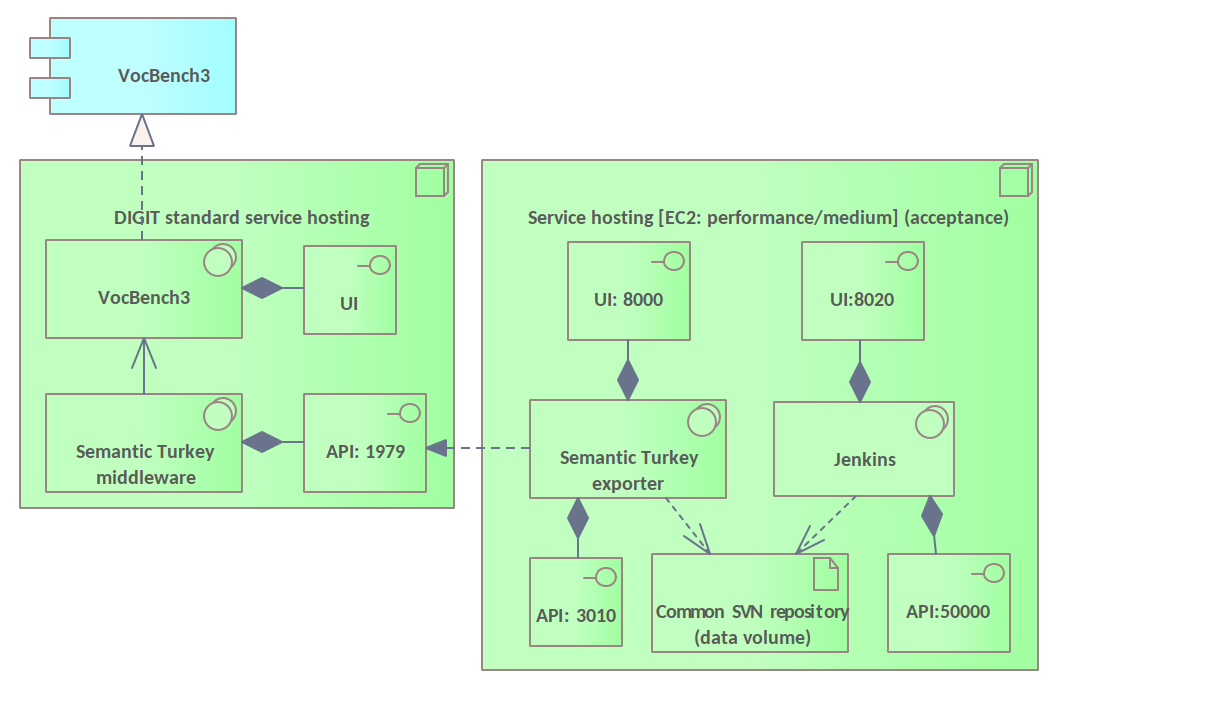
\includegraphics[width=\textwidth]{images/infra-setup/implementation.png}
		\caption{The technology components for exporting asset sources from VocBench3 into the common SVN repository}
		\label{fig:technology-view-implementation}
	\end{figure}
	
	Semantic Turkey exporter component shall be configured according to the Semantic Turkey installation offered by DIGIT (port, address and access rights). This component exposes a user interface and an API which allow exporting a selected project from VocBench3 and committing it into the common SVN component. If such component is missing, this operation can be performed manually until later implementation is available in place. 
	
	An instance of Jenkins automation server should be deployed and configured to listen to changes in the common SVN repository on preselected projects. It can be configured through the user interface or configuration files at the runtime. It also must be configured to trigger execution of RDF differ, RDF validator and RDF fingerprinter on the exported asset(s) and other configurations as necessary. Once an export is committed into the SVN repository Jenkins will automatically trigger chain execution of the pre-configured services. 
	
	The deployment organisation of the validation, diffing and fingerprinting services is described in the next section. 
	
	%This functionality of listening for changes in the SVN repository and firing other services is currently implemented in the legacy workflow component. 
	
	\section{Validation services}
	\label{sec:technology-view-validation}
	
	In this section we explain how SHACL validation, RDF fingerprinting and RDF differ components are deployed illustrated in Figure \ref{fig:technology-view-validation}. Each of the tree components is realised by a software component with a generic name of the function it realises: RDF validator, RDF differ and RDF fingerprinter. Each of these software components exposes two interfaces: one is the user interface and another is an API. The API represents the potential for being operated by an automation server such as Jenkins or an service orchestrator like Camunda. We omit to picture the hosting EC2 node as all the mentioned elements belong to it making it redundant in the diagram.
	
	\begin{figure}[!h]
		\centering
		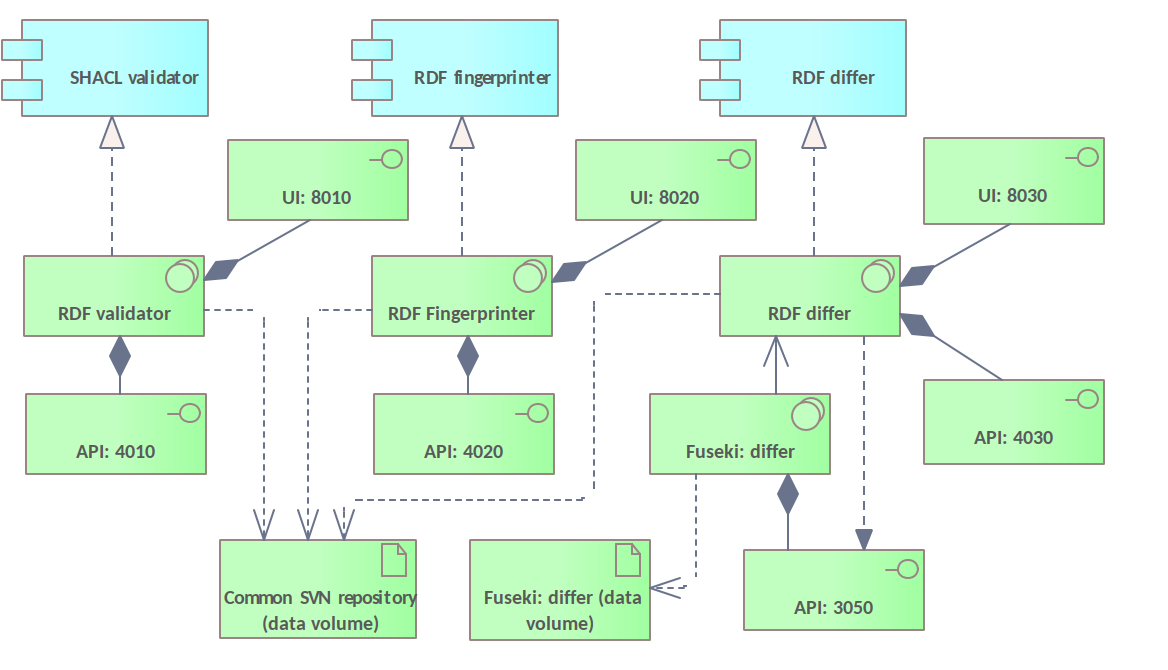
\includegraphics[width=\textwidth]{images/infra-setup/validation v2.png}
		\caption{The technology components for generation of assessment artefacts}
		\label{fig:technology-view-validation}
	\end{figure}

	The RDF validator, RDF fingerprinter and RDF differ are deployed as Docker containers and all have access to the common SVN repository volume. Doing so grants direct access to the stored files and provides the possibility to write and commit the results of their execution. For example the SHACL validator can access a file in the repository and write the validation report into the repository, next to the validated file. The RDF differ, in a similar manner, can load two versions of the same file from the common repository and compute the diff between them writing it back next to the latest version of it. The same holds for the RDF fingerprinter. 
	
	The RDF differ, does not run alone, it requires an instance of a running triple store, and in this case we choose Fuseki as it is a popular open source triple store. Another triple store can be chosen at a later stage. The reason why a triple store is necessary in the first place is that the RDF diffing operation is based on a series of SPARQL queries which can be executed only in a triple store. So in Figure \ref{fig:technology-view-validation} ``Fuseki:differ'' software is a Fuseki instance serving the RDF differ exclusively and is accessible through its API at pre-configured ports. The Fuseki instance persists its data outside the container in a dedicated volume mounted to it. 
	
	The port configuration suggested here is selected to be conflict-free and does not constitute a hard requirement and can be changed as the situation requires.
	
	A similar requirement hold for the RDF fingerprinter: a dedicated Fuseki triple store is necessary to ensure full functionality. 
	
	The RDF validator is implemented based on RDF Unit engine \citep{rdfunit-kontokostasDatabugger}. It does not have external dependencies and can validate an RDF file or a SPARQL endpoint. This makes it quite versatile because it is makes possible to execute validation operations both, on files stored in SVN common repository and on SPARQL endpoints storing intermediary data of ETL workflows and processes explained in the next section. 
	
	\section{Transformation services}
	\label{sec:technology-view-transformation}
	
	This section covers the software components necessary in the release stage when the RDF asset sources are transformed into various release artefacts. The infrastructure components and their interrelations are presented in Figure \ref{fig:technology-view-transformation}. 
	
	\begin{figure}[!h]
		\centering
		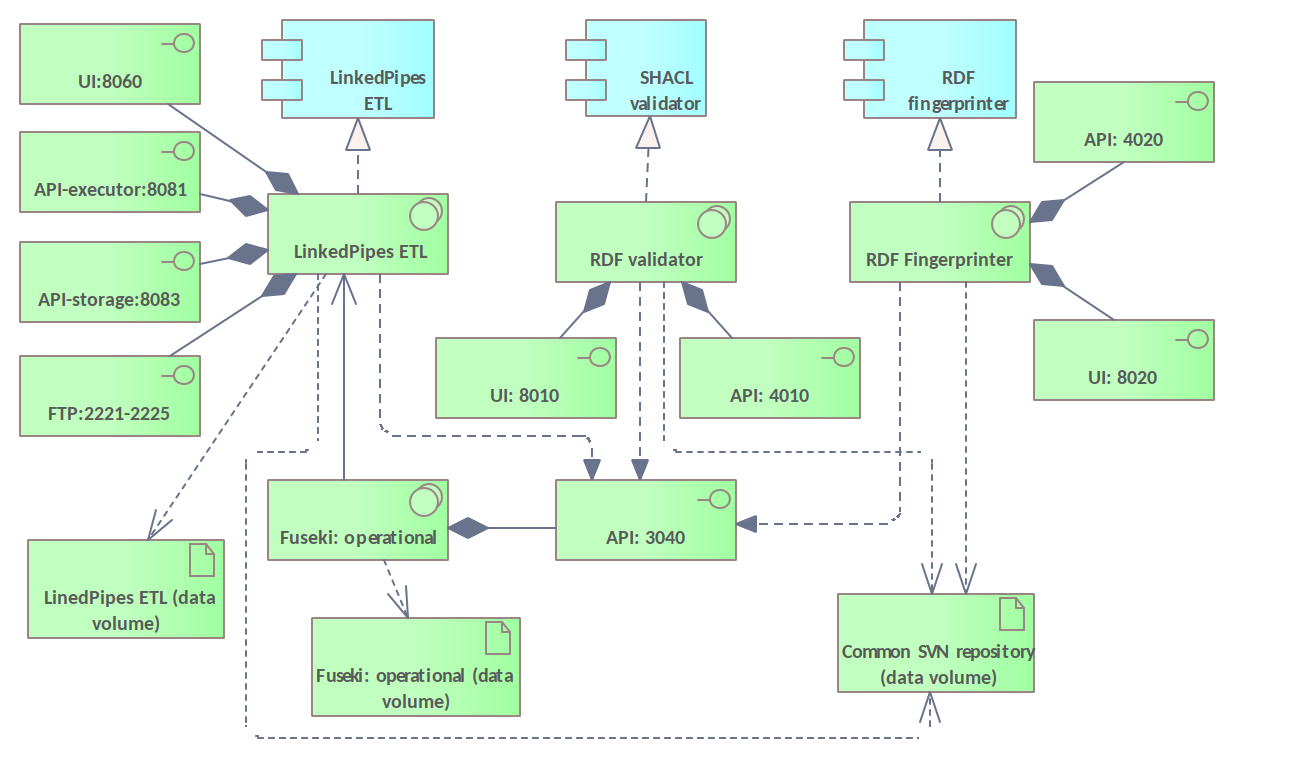
\includegraphics[width=.9\textwidth]{images/infra-setup/transformation.png}
		\caption{The technology components organisation for generation of release artefacts}
		\label{fig:technology-view-transformation}
	\end{figure}

	The key element is the LinkedPipes ETL application component (in light blue on the top of the diagram), which realises the RDF-based transformation and conversion of data. It is realised by a software element with the same name (in green below). This software exposes four technology interfaces, one of which is a user interface and the other three are technical APIs. In particular, the FTP interface is useful for debugging transformation processes while the other two for triggering and controlling the transformation process executor and the storage controller. LinkedPipes ETL can be deployed as a single container or as four separate containers, that depends on the original packaging of the software. 
	
	LinekdPipes ETL shall use the externally mounted SVN repository that serves as source for the transformation processes inputs and a place to write the final outcomes. For execution of the intermediary transformation operations and processing it needs another volume which is mounted to it. In addition it uses also a triple store for the same, operational, reasons. We propose to use a Fuseki instance dedicated to LinkedPipes ETL operations, which we call ``Fuseki: operational''. This Fuseki instance also shall use an externally mounted data volume for convenience and ease of management. 
	
	As explained in Section \ref{sec:release-new}, the transformation processes need to be controlled. Therefore the validation services described above are repeated here again to show the connection with the transformation service. The validation services have access to the ``Fuseki: operational'' instance and to the common SVN repository. Like this, a validation procedure can be triggered at any stage of the transformation process. The RDF differ is omitted from this figure because it is relevant in verifying the content implementation completeness and correctness and required human involvement. The SHACL validation and fingerprinting services can be used in a fully automated and semi-automated scenarios, and requiring little to no human intervention.
		
		
% 	\section{Reporting services}
% 	\label{sec:technology-view-reporting}
	
% 	This section covers the software components necessary for producing human readable reports on various aspects in asset publishing life-cycle. The infrastructure components and their interrelations are presented in Figure \ref{fig:technology-view-reporting}. 
	
% 	\begin{figure}[!h]
% 		\centering
% 		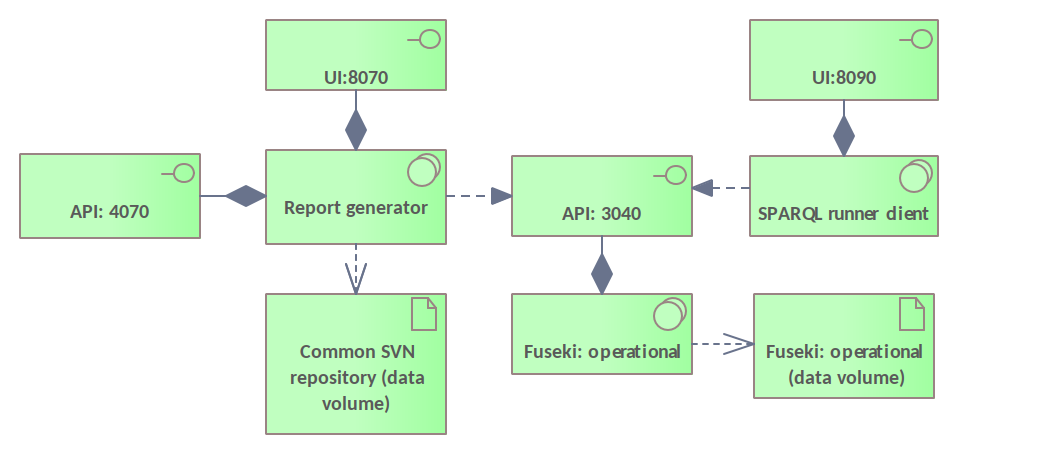
\includegraphics[width=.8\textwidth]{images/infra-setup/reporting.png}
% 		\caption{The technology components for generation of human readable artefacts}
% 		\label{fig:technology-view-reporting}
% 	\end{figure}
	
% 	The report generator is a software component which generates various reports in human readable formats such as HTML, PDF, Excel, DOCX. It does so by the virtue of predefined templates and by accessing data from the common SVN repository and from the Fuseki operational triple store. It exposes an user interface but can also access via an API.
	
% 	A very useful tool, especially fro the technical staff is a SPARQL client which can be used to execute SPARQL queries directly on SPARQL endpoints and display the results. We call it ``SPARQL runner client''. This software comes in handy when predefined queries need to be executed remotely in an automated or manual fashion outside the triple store facilities.
	
	
	\section{Service orchestration}
	\label{sec:technology-view-orchestration}
	
	This section covers the software components necessary for service orchestration across all steps of the asset publishing life-cycle. Adoption of a service orchestration application component was discussed in Section \ref{sec:implementation-application}. The infrastructure components and their interrelations are presented in Figure \ref{fig:technology-view-orchestration}. 
	
	\begin{figure}[!h]
		\centering
		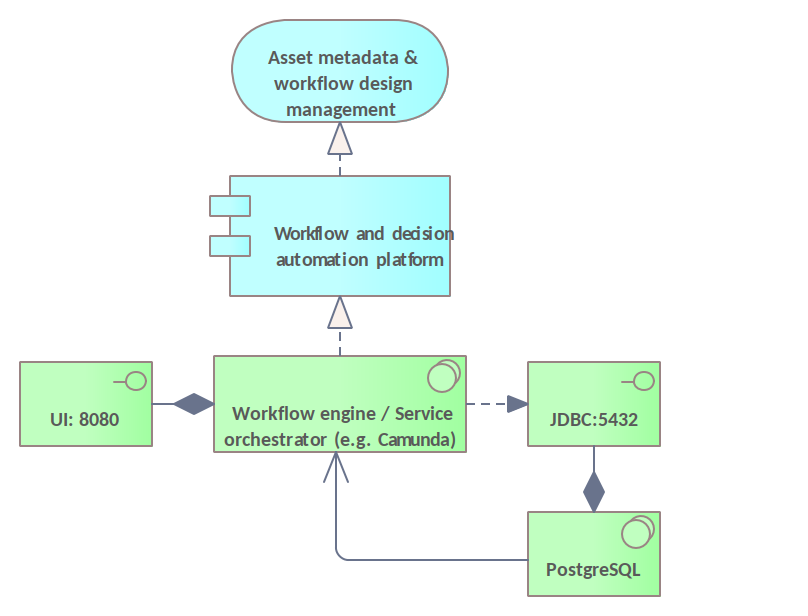
\includegraphics[width=.8\textwidth]{images/infra-setup/orchestration.png}
		\caption{The technology components for generation of human readable artefacts}
		\label{fig:technology-view-orchestration}
	\end{figure}

	In system administration, orchestration is the automated configuration, coordination, and management of computer systems and software. This can be done by designing and then executing a BPMN process. Business Process Model and Notation (BPMN) is a graphical representation for specifying business processes in a business process model. The objective of BPMN is to support business process management, for both technical users and business users, by providing a notation that is intuitive to business users, yet able to represent complex process semantics.

	We propose deployment of an instance of Camunda BPM server (or alike), which ships with tools for creating workflow and decision models, operating deployed models in production, and allowing users to execute workflow tasks assigned to them. It provides a BPMN compliant workflow engine and a Decision Model and Notation (DMN) compliant decision engine. 
	
	To support its functionality, Camunda needs a PostgreSQL database, which can be deployed in a sibling Docker container. Once Camunda BPM is deployed, BPMN workflows can be designed to access and trigger any services available on the AWS instances or any standard services offered by DIGIT. This will result in business staff being able to follow and execute entirely these workflows because the technicalities will be entirely hidden. 
		
	